% -*- LaTeX -*- %%%%%%%%%%%%%%%%%%%%%%%%%%%%%%%%%%%%%%%%%%%%%%%%%%%%%%
%
% Template for scribing COMP163 - Computational Geometry 
%
% Spring, 2004
%
%%%%%%%%%%%%%%%%%%%%%%%%%%%%%%%%%%%%%%%%%%%%%%%%%%%%%%%%%%%%%%%%%%%%%%
%**start of header 

\documentclass [12pt]{article}
\usepackage{epsfig}
\usepackage{enumitem}
\usepackage{amsmath}
\usepackage[color, leftbars]{changebar}

\usepackage{caption}
\usepackage{subcaption}


\setlength{\textwidth}{6.5in}
\setlength{\textheight}{9in}
\setlength{\oddsidemargin}{0in}
\setlength{\evensidemargin}{0in}
\setlength{\topmargin}{-0.5in}

\setlength{\parindent}{0pt}

\newtheorem{theorem}{Theorem}[section]
\newtheorem{definition}[theorem]{Definition}
\newtheorem{claim}[theorem]{Claim}
\newtheorem{lemma}[theorem]{Lemma}
\newtheorem{proof}[theorem]{Proof}

\newlength{\toppush}
\setlength{\toppush}{2\headheight}
\addtolength{\toppush}{\headsep}

\usepackage{hyperref}
\hypersetup{
    colorlinks=true,
    linkcolor=blue, % was previously black
    filecolor=magenta,
    urlcolor=blue,
    pdftitle={Template}
}
\urlstyle{same}

%\doheading{2}{title}{Last Revised: January, 2004}
%\htitle{title}

\def\subjnum{Comp 163}
\def\subjname{Computational Geometry}

\def\doheading#1#2#3{\vfill\eject\vspace*{-\toppush}%
  \vbox{\hbox to\textwidth{{\bf} \subjnum: \subjname \hfil Amy Bui}%
    \hbox to\textwidth{{\bf} Tufts University, Fall 2022 \hfil#3\strut}%
    \hrule}}

\newcommand{\htitle}[1]{\vspace*{3.25ex plus 1ex minus .2ex}%
\begin{center}
{\large\bf #1}
\end{center}} 

%%%%%%%%%%%%%%%%%%%%%%%%%%%%%%%%%%%%%%%%%%%%%%%%%%%%%%%%%%%%%%%%%%%

\begin{document}
\doheading{2}{title}{HW 3} 
% \htitle{Homework 1}
% \bigskip 
% \bigskip 
%%%%%%%%%% begin text after this line %%%%%%%%%%%%%%

    %%%%%%%%%%%%%%%%%%%%%%%%%%%%%%%%%%%%%%%%%%%%%%%%%%%%%%%%%%%%%%%%%%%%%%%%%
    \section{Diameter and Width (O'Rourke)}
    \label{sec:one}
        % \footnote{hello world}
        \begin{enumerate}[label=\alph*.]
            \item For a set $S$ of points, convex hull $\mathcal{CH}(S) \subseteq S$. The diameter of $S$ is given by two vertices in $\mathcal{CH}(S)$. I prove this by contradiction. Suppose there are two points $i, j \in S$; we consider $i \notin \mathcal{CH}(S)$ and $j \in \mathcal{CH}(S)$, and let $d$ be the length of $\overline{i\ j}$ and diameter of $S$. Since $i$ is not on the convex hull, there must exist a point $k$ ``further out'' from $i$ where $k\in \mathcal{CH}(S)$ where the length of $\overline{j\ k}$ is greater than $d$. Therefore, $d$ cannot be the diameter. The same can be true when $i \in \mathcal{CH}(S)$ and $j \notin \mathcal{CH}(S)$, as well as $i, j \notin \mathcal{CH}(S)$. Therefore the diameter must be a $d$ for $\overline{i\ j}$ where $i, j \in \mathcal{CH}(S)$.
            
            \item Support lines lie tangent to all $i\in \mathcal{CH}(S)$. From the previous problem, there exists $i, j \in S$ such that their distance is the max distance in $S$ and therefore $i, j\in \mathcal{CH}(S)$. And since they are on the convec hull, there exists support lines for each; let $\ell_i$ be the support line at $i$ that is perpendicular to $\overline{i\ j}$, and let $\ell_j$ be the support line at $j$ that is perpendicular to $\overline{i\ j}$. Since $\ell_i$ and $\ell_j$ are both perpendicular to the same line, they are parallel. Their distance is given by the distance of $\overline{i\ j}$, which is also the length of the diameter of $S$. Therefore, the distance between these parallel support lines is the diameter of $S$,
       
            \item Let $p_i, p_j\in \mathcal{CH}(S)$ be two extreme points (leftmost and rightmost, etc.). They are trivially antipodal because they are the furthest apart in the set, and there can exist parallel support lines $\ell_i$ and $\ell_j$, given above. 
            
            Calculate the angles given by $\ell_i$ and $\overline{p_i\ p_{i+1}}$, and by $\ell_j$ and $\overline{p_j\ p_{j+1}}$ (where the angle of rotation is counterclocwise). Let $a$ be the smaller of the two angles. In the ccw direction, rotate $\ell_i$ and $\ell_j$ by $a$ degrees until the line that made the smaller angle is tangent with it's vertex and the next vertext on the hull. For this example, let $\ell_i$ be that line, so it is now rotated to be tangent to $p_i$ and $p_{i+1}$. Since the newly rotated $\ell_i$ and $\ell_j$ are still parallel, we can report that $p_j$ and $p_{i+1}$ are antipodal. Since $\ell_i$ and $\overline{p_i\ p_{i+1}}$ created the smaller angle, $p_i := p_{i+1}$ (vice versa if the other line made the smaller angle). Repeat this process until the first antipodal pair is reencountered (rotated around once). 
            
            Since calculating rotations is constant and each point is visited once when we rotate around the hull, this algorithm runs in $O(n)$ time; space complexity is $O(1)$ because we are not storing extra data points other than $S$. The first pair of support lines of the trivially antipodal pair are given to be parallel; we can maintain throughout the algorithm that after each rotation, the two support lines remain parallel because they are rotated in the same direction at the same angle. And since the point about which the lines rotate change to the next point on the hull that each ``hits'', we can validate that the pairs reported are antipodal. 
           
            \item We can find the width using the same rotating algorithm as in part c, with the following modification: instead of reporting an antipodal pair, calculate the distance between the current parallel support lines, $\ell_i$ and $\ell_j$, and lets call it $w$. If $w$ is less than the current minimum width, $w_{\text{min}}$, when $w_{\text{min}} = w$. Report the $w_{\text{min}}$ after rotating around once. The time and space complexity, and correctness is the same as that of part c.
           
        \end{enumerate}
        
    \pagebreak
    % END %%%%%%%%%%%%%%%%%%%%%%%%%%%%%%%%%%%%%%%%%%%%%%%%%%%%%%%%%%%%%%%%%%%

    
    %%%%%%%%%%%%%%%%%%%%%%%%%%%%%%%%%%%%%%%%%%%%%%%%%%%%%%%%%%%%%%%%%%%%%%%%%
    \section{Minimum Area Triangle}
    \label{sec:two}

    \begin{enumerate}[label=\alph*.]
        \item $O(n^3)$ algorithm: For every triple $i, j, k\in S$, a triangle can be formed and it's area calculated in constant time. Report the smallest area found. There are $O(n^3)$ possible triples.
        
        \item Given $\overline{p_1 p_2}$, we can calculate its y-intercept $b$ and slope $m$. For all the other $n-2$ point $p_i\in S$, use $m$ to calculate the y-intercept $b_i$ given by the line characterized by $p_i$ and $m$. For each of those $n-2$ points, calculate the absolute difference $|b - b_i|$; we can then order these points by increasing value of this absolute difference. The point that forms the smallest area triangle with $\overline{p_1 p_2}$ is the one with the smallest absolute difference, i.e. the ``closest'' point to the line (Fig. \ref{fig:2b}). Since triangle area is given by $\frac{1}{2} \times $ base $\times$ height, and all these triangles have the same base, $\overline{p_1 p_2}$, the height will determine who has the smallest area. The smallest height is the length of the line perpendicular to $\overline{p_1 p_2}$ and includes the closest $p_i$. In the example of Fig. \ref{fig:2b}, point $j$ is the closest, as determined by its vertical distance (i.e. absolute difference in y-intercepts) from $\overline{p_1 p_2}$; it clearly gives the smallest height compared to the other points, and therefore yields the minimum area triangle with $\overline{p_1 p_2}$.
        

        \begin{figure}[h]
            \centering
            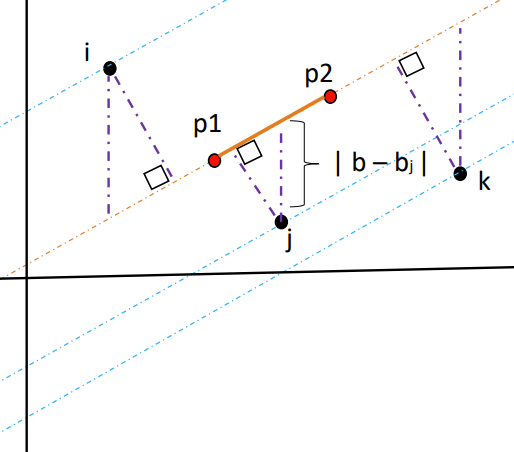
\includegraphics[width=0.7\textwidth]{images/2b.PNG}
            \caption {}
            \label{fig:2b}
        \end{figure}

        \pagebreak

        \item $o(n^3)$ duality and line sweeping algorithm: We can use Edelsbrunner, Welzl (1986) algorithm for LMSR that runs in $O(n^2 \log n)$ time and uses $O(n)$ space. For every point $p\in S$ given by $(p_x, p_y)$, create it's dual, $y = p_x\ x + p_y$. There are $O(n^2)$ stopping points we visit, given by the number of intersections in the dual; recall that an intersection in this dual represents the line segment in the primal that connects the two points that created the intersection in the dual. Using the status array, it will take $O(1)$ time to find the closest point (jump of 1) and calculate the area given by the two primal points that created the intersection in the dual, and the third point in the primal that gave us the closes line to this intersection point in the dual. This distance is preserved from the primal of the vertical distance from this third point to the segment. So from part b, we want to maintain only the triple that creates the smallest vertical distance from our sweeping. And finally, since the stopping data structure is a heap, it takes $O(\log n)$ to get to the next point in the sweep, so total runtime is $O(n^2 \log n)$. Space is $O(n)$ if we only maintain the stop points to the right of the sweep line and that are only those intersections of just current adjacent lines in the current sweep.\footnote{Jake helped clarified this algorithm in office hours.}
        
        % \pagebreak

        \item We can use the topological sweep algorithm in arrangement given Edelsbrunner, Guibas (1987), which has $O(n^2)$ time and $O(n)$ space because we are sweeping with a topological line, rather than with one that is always vertical. This paper also address solving the minimum area triangle problem with this topological sweep.
        
        Per Edelsbrunner, Guibas, at an elementary step, we are crossing over a vertex in the dual that represents a segment between two points in the primal. At this point in the algorithm, we know the vertex we just passed, the updated horizon tree gives us the the two edges that the topological line currently cuts, and the other two points of the region we entered can be calculated in constant time, because they are just the right endpoints of the two edges. No other edges should intersect the current region since the horizon is updated as such. With all this information, the area of the current region can be calculated and will correspond to the area given by the triangle of the three points in the primal that were transformed to the three lines that made the edge of the region. If the current triangle area is smaller than the current minimum area calculate, we update current minimum and continue the sweep. We report the final minimum area triangle and its three points in the end.\footnote{Jake went over possible modifications and the paper for this algorithm} 
       
    \end{enumerate}


    

    % \footnote{Jake walked through a correct algorithm for finding these bridges; with Alex and Stephanie.}

        
    \pagebreak
    % END %%%%%%%%%%%%%%%%%%%%%%%%%%%%%%%%%%%%%%%%%%%%%%%%%%%%%%%%%%%%%%%%%%%



    %%%%%%%%%%%%%%%%%%%%%%%%%%%%%%%%%%%%%%%%%%%%%%%%%%%%%%%%%%%%%%%%%%%%%%%%%
    \section{Double Wedges}
    \label{sec:three}

    \begin{enumerate}[label=\alph*.]
        \item Primal\footnote{Diane went over the difficulty of solving this in the primal}:
        
        Solving this problem in the primal yields a very complex algorithm:

        A line that intersects $t$ but no other segments in $S$ describes a line that exists ``between'' two separated parts of $S$, since it must not intersect any segments in $S$. Described another way, the solution line $L$ should be such that either: 
        
        1) if $\emptyset$ is on one half plane of $L$, and all of $S$ exist on the other side of $L$ without intersecting it, $t$ is not on or within a convex hull created from the line segments of $S$, or 

        2) if a non-empty part of $S$ exists on one half plane of $L$, and the other non-empty part exists on the other half plane of $L$ all without intersecting $L$, $t$ must be either a) not within either convex hulls of the two subsets, or b) not fully in only one of the two hulls. $L$ is then a line that intersects only the ``exposed'' segments of $t$ that is in the ``gap'' between the two hulls. 

        A way to solve this in the primal may be to enumerate every possible subset of $S$ and spend $O(n\log n)$ finding their convex hull, and test if $t$ passes or fails each of the above conditions. A set can have $2^n$ subsets, so runtime is a disaster, $O(2^n\ n \log n)$. 
        
        \item Dual\footnote{Diane and Jake went over a method of solving this problem in the dual.}:
        
        I describe an algorithm similar to the dual and sweep line algorithm described by Edelsbrunner, Welzl (1986), but for double wedges:
        
        For each line segment $\ell_i \in S$, using their endpoints ($i_A$ and $i_B$), make the transformation to the dual; each $\ell_i $ in the primal is then given by two intersecting lines ($T(i_A)$ and $T(i_B)$) in the dual, and the two regions bound by both lines on either side of the intersection point ($v_i$) are the double wedges. We also transform line $t$ to the dual. 

        We can then do a vertical sweep line across the dual. At a stopping point, moving up the stabbing line, we can note which of the lines $T(i_p)$ in the dual we are stabbing. Since the lines are ``paired'' with another line in the dual that belongs to a segment's other endpoint in the primal, we can tell when we are ``entering'' and ``leaving'' a region/wedge. When a segment of the sweep line is ``in a region'' bound by a wedge, then those points on the segment are in that wedge, the wedge corresponds to a segment in the primal $\ell_i$; when applying the same transformation on those sweep line points, but from the dual to the primal, each point $j$ corresponds to a line $T(j)$ in the primal that intersects $\ell_i$. So stabbing a wedge in the dual means we are intersecting the corresponding line segment in the primal. 
        
        Therefore, the goal is to find a region of the wedge corresponding to primal $t$ that does not overlap with any other wedges, i.e. the sweep line encounters a point such that it has a segment that is only in $t$'s wedge. If the sweep completes without encountering such a region, then a line that intersects $t$ but intersects no other segments in $S$ does not exist. If such a region is the dual is encountered, using any point in that subsegment of the sweep line but not the endpoints that intersects the lines of any wedges, we can transform that dual point $k$ (given by ($k_A, k_B$)) to a line in the primal $T(k) = y = k_A\ x + k_B$, and report this line as a solution.

        Again, we are stopping at $O(n^2)$ intersection points; however, it takes $O(n)$ at each stopping point to examine the $n$ stabbing points of the sweep line to determine which regions/wedges a subsegment of the sweep line overlaps, and it takes $O(\log n)$ to get the next stopping point, so the runtime is $O(n^3 \log n)$. It can still use $O(n)$ space if we only maintain the intersection points of adjacent lines we are stabbing.
       
    \end{enumerate}


    \pagebreak
    % END %%%%%%%%%%%%%%%%%%%%%%%%%%%%%%%%%%%%%%%%%%%%%%%%%%%%%%%%%%%%%%%%%%%



    %%%%%%%%%%%%%%%%%%%%%%%%%%%%%%%%%%%%%%%%%%%%%%%%%%%%%%%%%%%%%%%%%%%%%%%%%
    \section{Project}
    \label{sec:four}

    I emailed Diane about a project on line sweeping.

    % \begin{enumerate}[label=\alph*.]
    %     \item 
       
    % \end{enumerate}
    
        
    % \pagebreak
    % END %%%%%%%%%%%%%%%%%%%%%%%%%%%%%%%%%%%%%%%%%%%%%%%%%%%%%%%%%%%%%%%%%%%




    %%%%%%%%%%%%%%%%%%%%%%%%%%%%%%%%%%%%%%%%%%%%%%%%%%%%%%%%%%%%%%%%%%%%%%%%%
    

    % \pagebreak
    % END %%%%%%%%%%%%%%%%%%%%%%%%%%%%%%%%%%%%%%%%%%%%%%%%%%%%%%%%%%%%%%%%%%%



\begin{thebibliography}{1}
    \bibitem[1]{officehours}Jake and Diane's office hours, classmates: Stephanie, Alex, Anju with homework problem discussions.
    \bibitem[2]{berg08}Mark de Berg, Otfried Cheong, Marc van Kreveld, and Mark Overmars. 2008. Computational Geometry: Algorithms and Applications (3rd ed. ed.). Springer-Verlag TELOS, Santa Clara, CA, USA.
    \bibitem[3]{edelwel}H. Edelsbrunner and L.J Guibas, \href{https://www.sciencedirect.com/science/article/pii/002200008990038X}{``Topological Sweep an Arrangement''}. Journal of Computer and System Sciences. 38:164-194. 1989.
\end{thebibliography}
%%%%%%%%%%%%%%%%%%%%%%%%%%%%%%%%%%%%%%%%%%%%%%%%%%%%%%%%%%%%%%%%%%%%%%
\end{document}
%%%%%%%%%%%%%%%%%%%%%%%%%%%%%%%%%%%%%%%%%%%%%%%%%%%%%%%%%%%%%%%%%%%%%%

